%!TEX encoding = UTF-8 Unicode  
\documentclass{article}  
\usepackage{xeCJK}
\setCJKmainfont[BoldFont=STZhongsong, ItalicFont=STKaiti]{STSong}
\setCJKsansfont[BoldFont=STHeiti]{STXihei}
\setCJKmonofont{STFangsong}
\usepackage{graphicx}

\begin{document}  

\title{稀疏矩阵}
\date{}

\maketitle



就像在上一节描述的一样,标准的离散化的偏微分方程往往会伴随着一个庞大的且稀疏的矩阵。稀疏矩阵可以被模糊的描述为一个具有非常少的非零元的矩阵。但是,事实上,当特殊的技巧需要利用到大量的非零元以及它们的位置时,一个矩阵是可以被稀疏化的。这些稀疏化矩阵的技巧是从不储存零元的想法开始的。一个关键的问题是制定能够适合于高效地使用不论是直接还是迭代的标准计算方法的存储稀疏矩阵的数据结构。这一章节将简介稀疏矩阵,它们的属性、呈现,以及用以存储它们的数据结构。
\newline\newline

\textbf{3.1介绍}
\newline\newline
利用一个矩阵中的零元以及它们的位置的自然的想法最初是由在不同学科的工程师们提出的。在涉及带状矩阵的简单地例子中,特殊的技巧直接的被发明了。在20世纪60年代研发电子网络的电子工程师们是最早的去利用稀疏性来对于具有特殊结构的矩阵解决一般稀疏线性系统。对于稀疏矩阵技巧而言,最主要也是最早需要解决的问题是去设计一个在线性系统中得直接求解算法。这些算法需要是可以接受的,在存储和计算效率上。直接的稀疏算法可以被用于计算那些庞大的难以被稠密算法来实现的问题。
\newline\newline\newline\newline\newline\newline\newline\newline

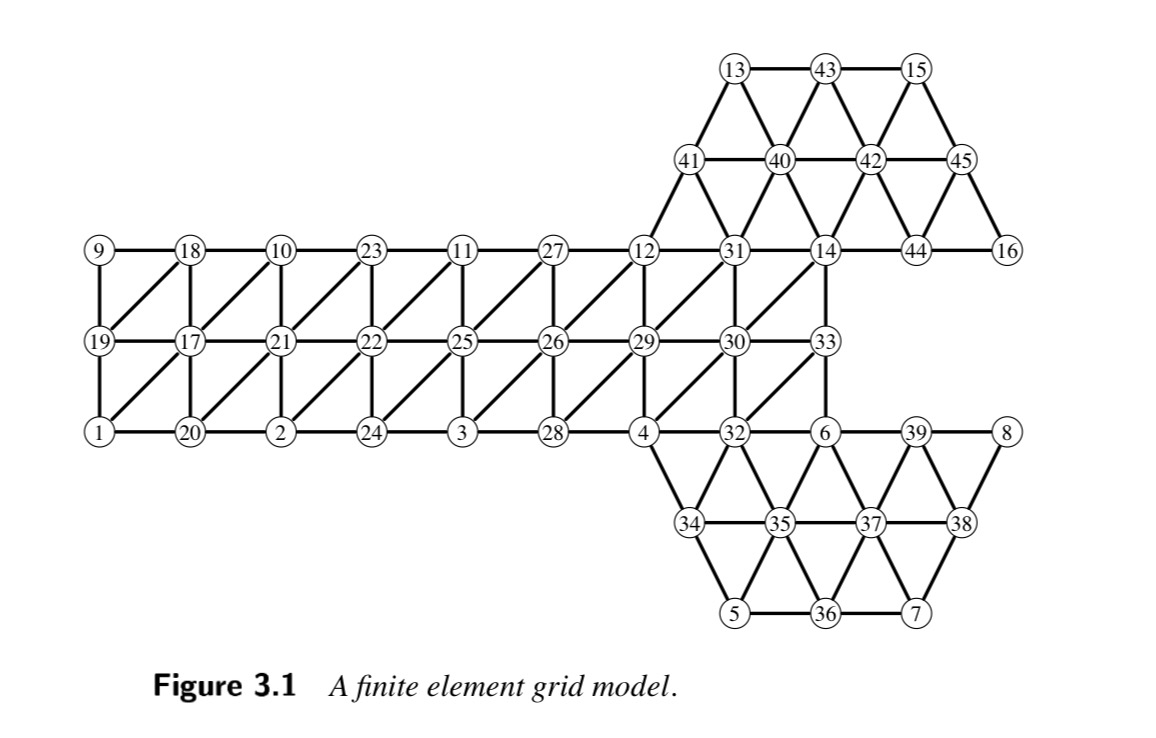
\includegraphics[scale=0.25]{3_1.png}

基本上,有两个明显的类别的稀疏矩阵,结构化的和非结构化的。一个结构化的矩阵是指一个非零元的位置形成某个规律的矩阵,通常这些非零元在对角线附近。要不然,这些非零元会在相同大小的块内(稠密子矩阵),而这也会形成一个规律,通常这些非零元在对角线(块)附近。一个具有着不规则位置的非零元的矩阵会被称作是非结构化的。最好的一个结构化的矩阵的例子是一个只有着少量对角元的矩阵。网格上的有限差分矩阵,就像上一节中提到的,是典型的具有着规律结构的例子。大部分的对于复杂几何的有限元和有限体积技巧会导致非结构化的矩阵。图3.2展示了一个与图3.1所呈现的有限元网格问题的一个小规模的非结构化的矩阵。
\newline

这两种类型的矩阵间的区别可能并不会明显的影响到直接求解技巧,而且,在过去,它并没受到过多的关注。但是,对于迭代求解方法,这个区别是很重要的。在这些方法中,最基本的运算之一是矩阵向量求积。在高性能计算机上,这些运算受规则化程度的影响很大。比如,在向量计算机上,理想的是存储对角元,但是更通常的设计可能会较慢,因为他们需要间接寻址。
\newline

下一节将讨论用图来呈现稀疏矩阵。
\newline\newline\newline\newline\newline\newline
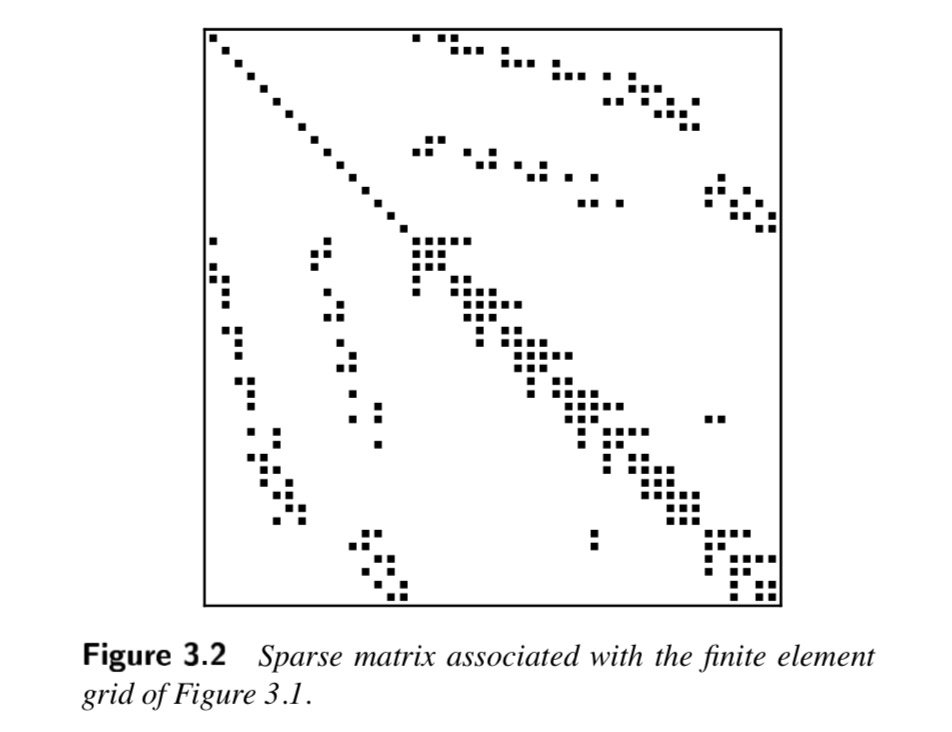
\includegraphics[scale=0.4]{3_2.png}
\newline\newline
\textbf{3.2图论}
\newline
图论是用来表示稀疏矩阵结构的一个理想的工具,因此,在稀疏矩阵技巧中,它扮演着一个主要的角色。例如,图论是用于解决并行稀疏高斯消除和预处理技术的关键。在下一节中,将讨论图的一般特性,以及它们在有限元和有限差分矩阵中得应用。

\textbf{3.2.1图与邻接图}
记住一个图由两个集合定义,一个顶点集合$V =\{v_1,v_2,\cdots,v_n\}$和一个边的集合E,E是由点对$(v_i,v_j)$组成的,$v_i,v_j$都是V中的元素,换而言之,$E\subseteq V\times V$。这个图$G=(V,E)$通常被平面内的一系列的被边联系的点的向量来表示。这个图被用来描述集合V中元素间的关系。例如,V可以被用来描述世界上的主要城市。线就是两个城市间的直达航线。那么这个图就会描述这样一个关系“在城市A和城市B间存在一条直达航线”。在这个特殊的例子中,二元关系很可能是对称的,换而言之,如果有一条A到B的直达航线,那么也有一条B到A的直达航线。在这样的情形中,图被称作是无向的,用以与通常的有向图相对。
  \newline\newline\newline\newline\newline\newline
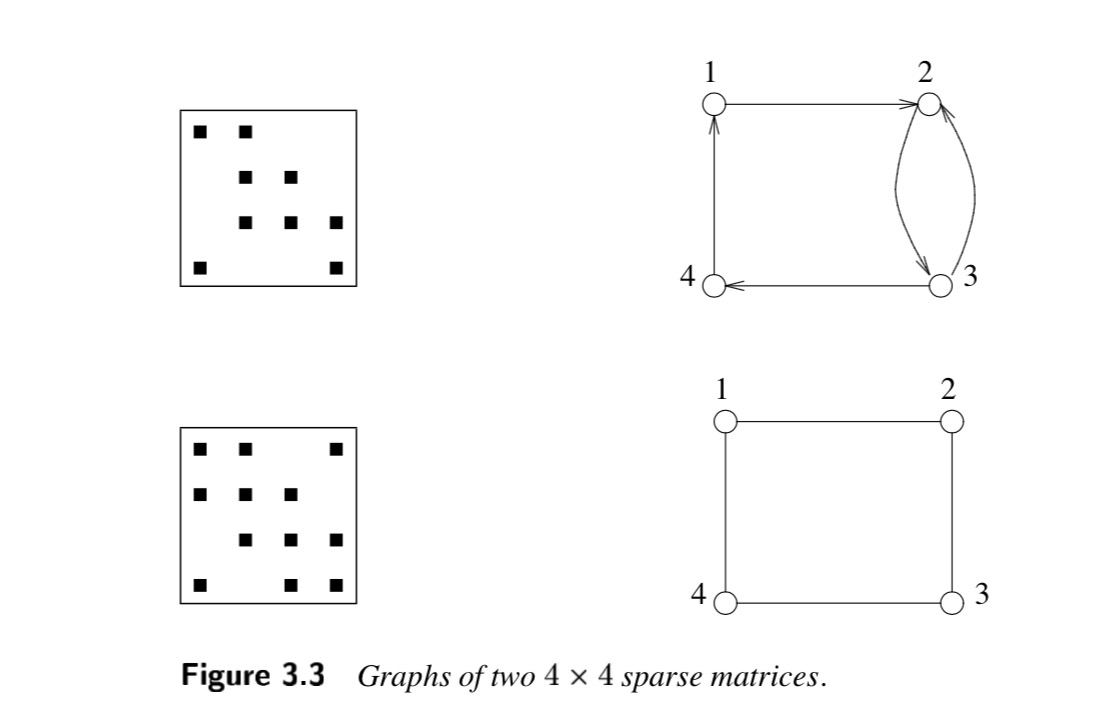
\includegraphics[scale=0.25]{3_3.png}
\newline\newline
回到稀疏矩阵,稀疏矩阵的邻接图是一个图$G=(V,E)$,V中得n个顶点代表n个未知数。



\end{document}  
